\documentclass{article}


%%%%%%%%%%%%%%%%%%%%%%%%%%%%%%%%%%%%%%%%%%%%%%%%%%%%%%%%%%%%%%%%%%%%%%%%%
\pagestyle{plain}                                                      %%
%%%%%%%%%% EXACT 1in MARGINS %%%%%%%                                   %%
\setlength{\textwidth}{6.5in}     %%                                   %%
\setlength{\oddsidemargin}{0in}   %% (It is recommended that you       %%
\setlength{\evensidemargin}{0in}  %%  not change these parameters,     %%
\setlength{\textheight}{8.5in}    %%  at the risk of having your       %%
\setlength{\topmargin}{0in}       %%  proposal dismissed on the basis  %%
\setlength{\headheight}{0in}      %%  of incorrect formatting!!!)      %%
\setlength{\headsep}{0in}         %%                                   %%
\setlength{\footskip}{.5in}       %%                                   %%
%%%%%%%%%%%%%%%%%%%%%%%%%%%%%%%%%%%%                                   %%
\newcommand{\required}[1]{\section*{\hfil #1\hfil}}                    %%
\renewcommand{\refname}{\hfil References Cited\hfil}                   %%
\bibliographystyle{plain}                                              %%
%%%%%%%%%%%%%%%%%%%%%%%%%%%%%%%%%%%%%%%%%%%%%%%%%%%%%%%%%%%%%%%%%%%%%%%%%

\usepackage{graphicx}

\pagestyle{plain}

\begin{document}

\large

\vbox{}
\begin{figure}[!ht]
%\hspace{-4mm}

\includegraphics[width=5cm]{logo.png}
\vspace{4mm}
\end{figure}

\centerline{\huge \bf Postprocessor}
\vspace{6mm}
\noindent
This help will guide you through NCLab's Postprocessor (PP).

\subsection*{Copyright and Restricted Use Notice}

The Postprocessor (PP) is part of the Networked Computing Laboratory (NCLab) and its sole 
purpose is to facilitate visualization and postprocessing of results of finite element 
calculations in NCLab. PP is a closed-source code that is copyrighted by FEMhub Inc. Copying 
and any use outside of NCLab is strictly prohibited.

\subsection*{Launching PP}

PP can be launched from any Python worksheet in NCLab by issuing 

\begin{verbatim}
lab.postprocessor().
\end{verbatim}
After PP launches, right-click in the work area and a menu will appear:\\

\begin{figure}[!ht]
\begin{center}
%\hspace{-4mm}
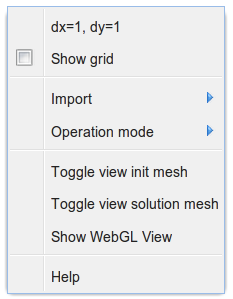
\includegraphics[width=4.5cm]{pp-menu.png}
\end{center}
\vspace{-4mm}
\caption{Postprocessor's menu.}
\end{figure}


\subsection*{Overview of Menu Functions}

In the order of appearance, the menu functions do the following:
\begin{itemize}
\item Grid spacing: Sets grid spacing in the x and y directions.
\item Show grid: Turns on and off grid display.
\item Import: When you are importing you have two possibilities how to do it now. First is to copy paste the content of file into a text area that is up or you can choose file form your local disk. Then click on import button. The following can be imported:
\begin{itemize}
\item Geometry: it loads geometry form geometry editor - it is used now for edge and sub-domain selection.
\item Init mesh: Initital mesh that comes from mesh editor - currently used just for visualization of initial mesh.
\item Solution: Imports sln.vtk files from hermes examples currently. It renders the solution and open debug window where you can see solution value in nearest vertex in solution mesh.
\item Problem UI - import Agros module file - opens UI for local variables and volume/surface integrals.
\end{itemize}
\item Operation mode:
\begin{itemize}
\item Point - for selecting points to discover point value of local variables.
\item Edge - when mouse click is performed nearest edges is selected - prepared for path integrals.
\item Subdomains - when mouse click is performed subdomain under mouse is selected.
\end{itemize}
\item Toggle view init mesh: Toggle visibility of init mesh.
\item Toggle view solution mesh: Toggle visibility of solution mesh.
\item Show WebGL View: Open new window with WebGL view.
\item Help: Launches this Help.
\end{itemize}



\subsection*{Known Bugs}

No known bugs at this time. Please report bugs to {\tt nclab-user@googlegroups.com}.
\end{document}

